% Created by tikzDevice version 0.12.3 on 2020-06-17 00:07:33
% !TEX encoding = UTF-8 Unicode
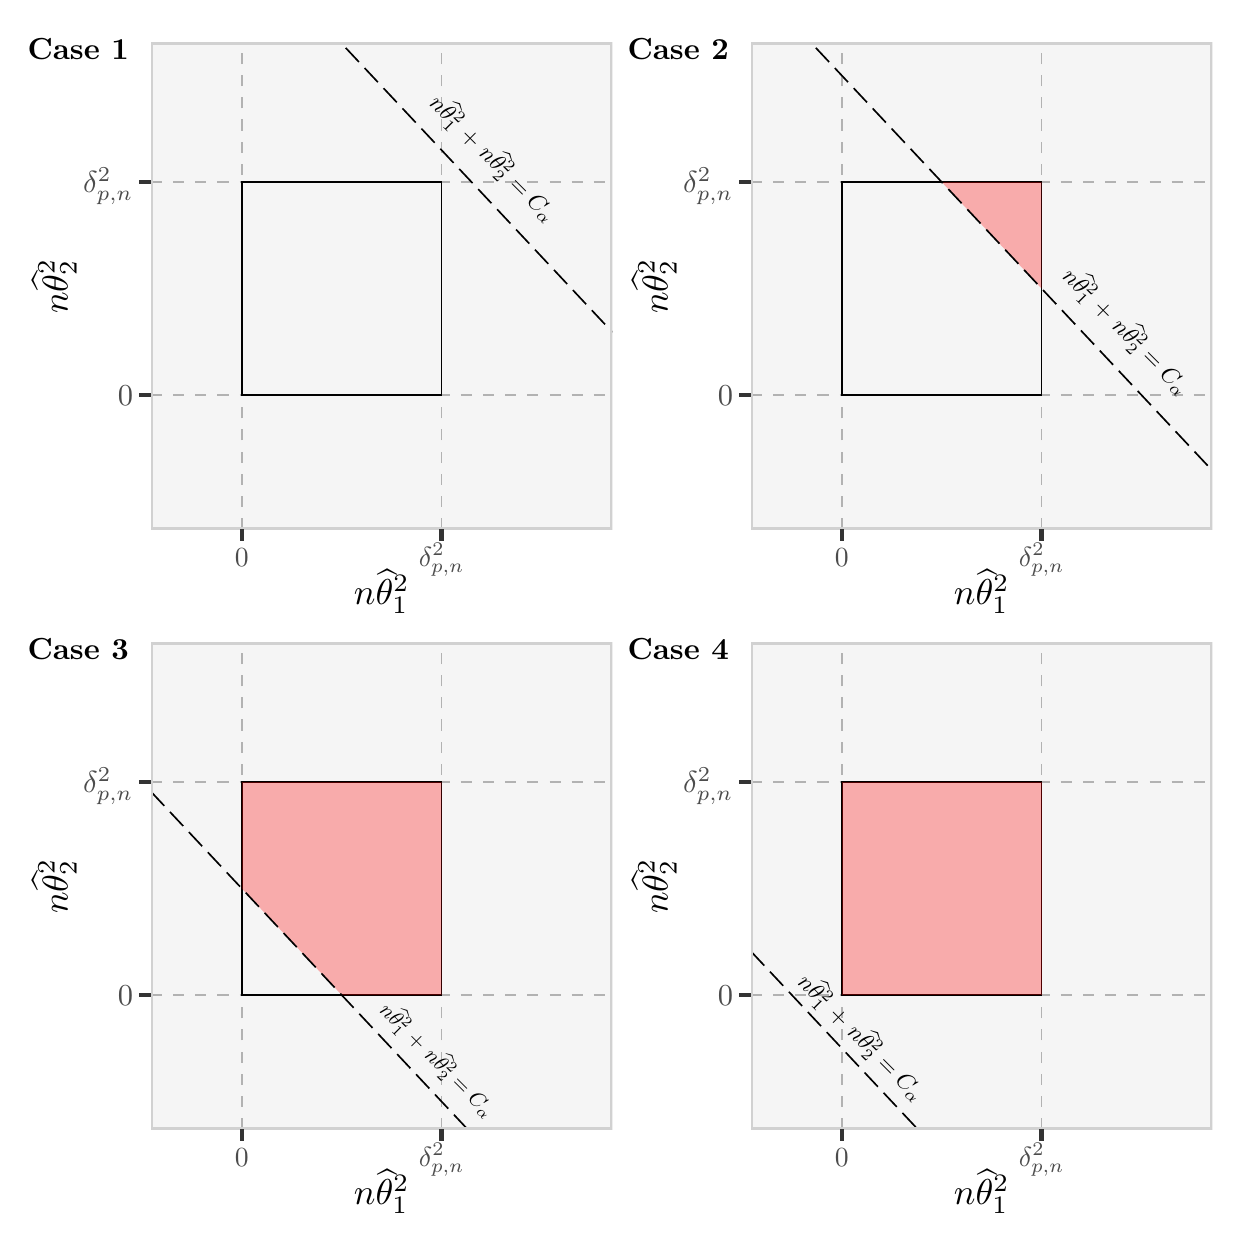
\begin{tikzpicture}[x=1pt,y=1pt]
\definecolor{fillColor}{RGB}{255,255,255}
\path[use as bounding box,fill=fillColor,fill opacity=0.00] (0,0) rectangle (433.62,433.62);
\begin{scope}
\path[clip] (  0.00,216.81) rectangle (216.81,433.62);
\definecolor{drawColor}{RGB}{255,255,255}
\definecolor{fillColor}{RGB}{255,255,255}

\path[draw=drawColor,line width= 0.6pt,line join=round,line cap=round,fill=fillColor] (  0.00,216.81) rectangle (216.81,433.62);
\end{scope}
\begin{scope}
\path[clip] ( 44.57,252.45) rectangle (211.31,428.12);
\definecolor{fillColor}{gray}{0.96}

\path[fill=fillColor] ( 44.57,252.45) rectangle (211.31,428.12);
\definecolor{drawColor}{gray}{0.70}

\path[draw=drawColor,line width= 0.6pt,dash pattern=on 4pt off 4pt ,line join=round] ( 44.57,300.84) --
	(211.31,300.84);

\path[draw=drawColor,line width= 0.6pt,dash pattern=on 4pt off 4pt ,line join=round] ( 44.57,377.80) --
	(211.31,377.80);

\path[draw=drawColor,line width= 0.6pt,dash pattern=on 4pt off 4pt ,line join=round] ( 77.41,252.45) --
	( 77.41,428.12);

\path[draw=drawColor,line width= 0.6pt,dash pattern=on 4pt off 4pt ,line join=round] (149.59,252.45) --
	(149.59,428.12);
\definecolor{drawColor}{RGB}{0,0,0}

\path[draw=drawColor,line width= 0.6pt,line cap=rect] ( 77.41,300.84) rectangle (149.59,377.80);

\path[draw=drawColor,line width= 0.6pt,dash pattern=on 7pt off 3pt ,line join=round] (108.07,433.62) -- (211.31,323.54);

\node[text=drawColor,rotate=-45.00,anchor=base,inner sep=0pt, outer sep=0pt, scale=  0.85] at (166.28,384.19) {$n \widehat{\theta}^2_1$ + $n \widehat{\theta}^2_2 = C_{\alpha}$};
\definecolor{drawColor}{gray}{0.82}

\path[draw=drawColor,line width= 1.7pt,line join=round,line cap=round] ( 44.57,252.45) rectangle (211.31,428.12);
\end{scope}
\begin{scope}
\path[clip] (  0.00,  0.00) rectangle (433.62,433.62);
\definecolor{drawColor}{gray}{0.30}

\node[text=drawColor,anchor=base east,inner sep=0pt, outer sep=0pt, scale=  1.10] at ( 38.10,297.05) {0};

\node[text=drawColor,anchor=base east,inner sep=0pt, outer sep=0pt, scale=  1.10] at ( 38.10,374.02) {$\delta_{p,n}^2$};
\end{scope}
\begin{scope}
\path[clip] (  0.00,  0.00) rectangle (433.62,433.62);
\definecolor{drawColor}{gray}{0.20}

\path[draw=drawColor,line width= 1.7pt,line join=round] ( 40.30,300.84) --
	( 44.57,300.84);

\path[draw=drawColor,line width= 1.7pt,line join=round] ( 40.30,377.80) --
	( 44.57,377.80);
\end{scope}
\begin{scope}
\path[clip] (  0.00,  0.00) rectangle (433.62,433.62);
\definecolor{drawColor}{gray}{0.20}

\path[draw=drawColor,line width= 1.7pt,line join=round] ( 77.41,248.18) --
	( 77.41,252.45);

\path[draw=drawColor,line width= 1.7pt,line join=round] (149.59,248.18) --
	(149.59,252.45);
\end{scope}
\begin{scope}
\path[clip] (  0.00,  0.00) rectangle (433.62,433.62);
\definecolor{drawColor}{gray}{0.30}

\node[text=drawColor,anchor=base,inner sep=0pt, outer sep=0pt, scale=  1.00] at ( 77.41,239.09) {0};

\node[text=drawColor,anchor=base,inner sep=0pt, outer sep=0pt, scale=  1.00] at (149.59,239.09) {$ \delta_{p,n}^2$};
\end{scope}
\begin{scope}
\path[clip] (  0.00,  0.00) rectangle (433.62,433.62);
\definecolor{drawColor}{RGB}{0,0,0}

\node[text=drawColor,anchor=base,inner sep=0pt, outer sep=0pt, scale=  1.30] at (127.94,225.18) {$n \widehat{\theta}_1^2$};
\end{scope}
\begin{scope}
\path[clip] (  0.00,  0.00) rectangle (433.62,433.62);
\definecolor{drawColor}{RGB}{0,0,0}

\node[text=drawColor,rotate= 90.00,anchor=base,inner sep=0pt, outer sep=0pt, scale=  1.30] at ( 14.45,340.28) {$n \widehat{\theta}_2^2$};
\end{scope}
\begin{scope}
\path[clip] (  0.00,  0.00) rectangle (433.62,433.62);
\definecolor{drawColor}{RGB}{0,0,0}

\node[text=drawColor,anchor=base west,inner sep=0pt, outer sep=0pt, scale=  1.10] at (  0.00,422.23) {\bfseries Case 1};
\end{scope}
\begin{scope}
\path[clip] (216.81,216.81) rectangle (433.62,433.62);
\definecolor{drawColor}{RGB}{255,255,255}
\definecolor{fillColor}{RGB}{255,255,255}

\path[draw=drawColor,line width= 0.6pt,line join=round,line cap=round,fill=fillColor] (216.81,216.81) rectangle (433.62,433.62);
\end{scope}
\begin{scope}
\path[clip] (261.38,252.45) rectangle (428.12,428.12);
\definecolor{fillColor}{gray}{0.96}

\path[fill=fillColor] (261.38,252.45) rectangle (428.12,428.12);
\definecolor{drawColor}{gray}{0.70}

\path[draw=drawColor,line width= 0.6pt,dash pattern=on 4pt off 4pt ,line join=round] (261.38,300.84) --
	(428.12,300.84);

\path[draw=drawColor,line width= 0.6pt,dash pattern=on 4pt off 4pt ,line join=round] (261.38,377.80) --
	(428.12,377.80);

\path[draw=drawColor,line width= 0.6pt,dash pattern=on 4pt off 4pt ,line join=round] (294.22,252.45) --
	(294.22,428.12);

\path[draw=drawColor,line width= 0.6pt,dash pattern=on 4pt off 4pt ,line join=round] (366.40,252.45) --
	(366.40,428.12);
\definecolor{drawColor}{RGB}{0,0,0}

\path[draw=drawColor,line width= 0.6pt,line cap=rect] (294.22,300.84) rectangle (366.40,377.80);
\definecolor{fillColor}{RGB}{255,0,0}

\path[fill=fillColor,fill opacity=0.30] (330.31,377.80) --
	(366.40,377.80) --
	(366.40,339.32) --
	cycle;

\path[draw=drawColor,line width= 0.6pt,dash pattern=on 7pt off 3pt ,line join=round] (277.96,433.62) -- (428.12,273.52);

\node[text=drawColor,rotate=-45.00,anchor=base,inner sep=0pt, outer sep=0pt, scale=  0.85] at (395.00,321.85) {$n \widehat{\theta}^2_1$ + $n \widehat{\theta}^2_2 = C_{\alpha}$};
\definecolor{drawColor}{gray}{0.82}

\path[draw=drawColor,line width= 1.7pt,line join=round,line cap=round] (261.38,252.45) rectangle (428.12,428.12);
\end{scope}
\begin{scope}
\path[clip] (  0.00,  0.00) rectangle (433.62,433.62);
\definecolor{drawColor}{gray}{0.30}

\node[text=drawColor,anchor=base east,inner sep=0pt, outer sep=0pt, scale=  1.10] at (254.91,297.05) {0};

\node[text=drawColor,anchor=base east,inner sep=0pt, outer sep=0pt, scale=  1.10] at (254.91,374.02) {$\delta_{p,n}^2$};
\end{scope}
\begin{scope}
\path[clip] (  0.00,  0.00) rectangle (433.62,433.62);
\definecolor{drawColor}{gray}{0.20}

\path[draw=drawColor,line width= 1.7pt,line join=round] (257.11,300.84) --
	(261.38,300.84);

\path[draw=drawColor,line width= 1.7pt,line join=round] (257.11,377.80) --
	(261.38,377.80);
\end{scope}
\begin{scope}
\path[clip] (  0.00,  0.00) rectangle (433.62,433.62);
\definecolor{drawColor}{gray}{0.20}

\path[draw=drawColor,line width= 1.7pt,line join=round] (294.22,248.18) --
	(294.22,252.45);

\path[draw=drawColor,line width= 1.7pt,line join=round] (366.40,248.18) --
	(366.40,252.45);
\end{scope}
\begin{scope}
\path[clip] (  0.00,  0.00) rectangle (433.62,433.62);
\definecolor{drawColor}{gray}{0.30}

\node[text=drawColor,anchor=base,inner sep=0pt, outer sep=0pt, scale=  1.00] at (294.22,239.09) {0};

\node[text=drawColor,anchor=base,inner sep=0pt, outer sep=0pt, scale=  1.00] at (366.40,239.09) {$ \delta_{p,n}^2$};
\end{scope}
\begin{scope}
\path[clip] (  0.00,  0.00) rectangle (433.62,433.62);
\definecolor{drawColor}{RGB}{0,0,0}

\node[text=drawColor,anchor=base,inner sep=0pt, outer sep=0pt, scale=  1.30] at (344.75,225.18) {$n \widehat{\theta}_1^2$};
\end{scope}
\begin{scope}
\path[clip] (  0.00,  0.00) rectangle (433.62,433.62);
\definecolor{drawColor}{RGB}{0,0,0}

\node[text=drawColor,rotate= 90.00,anchor=base,inner sep=0pt, outer sep=0pt, scale=  1.30] at (231.26,340.28) {$n \widehat{\theta}_2^2$};
\end{scope}
\begin{scope}
\path[clip] (  0.00,  0.00) rectangle (433.62,433.62);
\definecolor{drawColor}{RGB}{0,0,0}

\node[text=drawColor,anchor=base west,inner sep=0pt, outer sep=0pt, scale=  1.10] at (216.81,422.23) {\bfseries Case 2};
\end{scope}
\begin{scope}
\path[clip] (  0.00,  0.00) rectangle (216.81,216.81);
\definecolor{drawColor}{RGB}{255,255,255}
\definecolor{fillColor}{RGB}{255,255,255}

\path[draw=drawColor,line width= 0.6pt,line join=round,line cap=round,fill=fillColor] (  0.00,  0.00) rectangle (216.81,216.81);
\end{scope}
\begin{scope}
\path[clip] ( 44.57, 35.64) rectangle (211.31,211.31);
\definecolor{fillColor}{gray}{0.96}

\path[fill=fillColor] ( 44.57, 35.64) rectangle (211.31,211.31);
\definecolor{drawColor}{gray}{0.70}

\path[draw=drawColor,line width= 0.6pt,dash pattern=on 4pt off 4pt ,line join=round] ( 44.57, 84.03) --
	(211.31, 84.03);

\path[draw=drawColor,line width= 0.6pt,dash pattern=on 4pt off 4pt ,line join=round] ( 44.57,160.99) --
	(211.31,160.99);

\path[draw=drawColor,line width= 0.6pt,dash pattern=on 4pt off 4pt ,line join=round] ( 77.41, 35.64) --
	( 77.41,211.31);

\path[draw=drawColor,line width= 0.6pt,dash pattern=on 4pt off 4pt ,line join=round] (149.59, 35.64) --
	(149.59,211.31);
\definecolor{drawColor}{RGB}{0,0,0}

\path[draw=drawColor,line width= 0.6pt,line cap=rect] ( 77.41, 84.03) rectangle (149.59,160.99);
\definecolor{fillColor}{RGB}{255,0,0}

\path[fill=fillColor,fill opacity=0.30] ( 77.41,122.51) --
	( 77.41,160.99) --
	(149.59,160.99) --
	(149.59, 84.03) --
	(113.50, 84.03) --
	cycle;

\path[draw=drawColor,line width= 0.6pt,dash pattern=on 7pt off 3pt ,line join=round] ( 44.57,157.53) -- (192.31,  0.00);

\node[text=drawColor,rotate=-45.00,anchor=base,inner sep=0pt, outer sep=0pt, scale=  0.77] at (146.28, 58.68) {$n \widehat{\theta}^2_1$ + $n \widehat{\theta}^2_2 = C_{\alpha}$};
\definecolor{drawColor}{gray}{0.82}

\path[draw=drawColor,line width= 1.7pt,line join=round,line cap=round] ( 44.57, 35.64) rectangle (211.31,211.31);
\end{scope}
\begin{scope}
\path[clip] (  0.00,  0.00) rectangle (433.62,433.62);
\definecolor{drawColor}{gray}{0.30}

\node[text=drawColor,anchor=base east,inner sep=0pt, outer sep=0pt, scale=  1.10] at ( 38.10, 80.24) {0};

\node[text=drawColor,anchor=base east,inner sep=0pt, outer sep=0pt, scale=  1.10] at ( 38.10,157.21) {$\delta_{p,n}^2$};
\end{scope}
\begin{scope}
\path[clip] (  0.00,  0.00) rectangle (433.62,433.62);
\definecolor{drawColor}{gray}{0.20}

\path[draw=drawColor,line width= 1.7pt,line join=round] ( 40.30, 84.03) --
	( 44.57, 84.03);

\path[draw=drawColor,line width= 1.7pt,line join=round] ( 40.30,160.99) --
	( 44.57,160.99);
\end{scope}
\begin{scope}
\path[clip] (  0.00,  0.00) rectangle (433.62,433.62);
\definecolor{drawColor}{gray}{0.20}

\path[draw=drawColor,line width= 1.7pt,line join=round] ( 77.41, 31.37) --
	( 77.41, 35.64);

\path[draw=drawColor,line width= 1.7pt,line join=round] (149.59, 31.37) --
	(149.59, 35.64);
\end{scope}
\begin{scope}
\path[clip] (  0.00,  0.00) rectangle (433.62,433.62);
\definecolor{drawColor}{gray}{0.30}

\node[text=drawColor,anchor=base,inner sep=0pt, outer sep=0pt, scale=  1.00] at ( 77.41, 22.28) {0};

\node[text=drawColor,anchor=base,inner sep=0pt, outer sep=0pt, scale=  1.00] at (149.59, 22.28) {$ \delta_{p,n}^2$};
\end{scope}
\begin{scope}
\path[clip] (  0.00,  0.00) rectangle (433.62,433.62);
\definecolor{drawColor}{RGB}{0,0,0}

\node[text=drawColor,anchor=base,inner sep=0pt, outer sep=0pt, scale=  1.30] at (127.94,  8.37) {$n \widehat{\theta}_1^2$};
\end{scope}
\begin{scope}
\path[clip] (  0.00,  0.00) rectangle (433.62,433.62);
\definecolor{drawColor}{RGB}{0,0,0}

\node[text=drawColor,rotate= 90.00,anchor=base,inner sep=0pt, outer sep=0pt, scale=  1.30] at ( 14.45,123.47) {$n \widehat{\theta}_2^2$};
\end{scope}
\begin{scope}
\path[clip] (  0.00,  0.00) rectangle (433.62,433.62);
\definecolor{drawColor}{RGB}{0,0,0}

\node[text=drawColor,anchor=base west,inner sep=0pt, outer sep=0pt, scale=  1.10] at (  0.00,205.42) {\bfseries Case 3};
\end{scope}
\begin{scope}
\path[clip] (216.81,  0.00) rectangle (433.62,216.81);
\definecolor{drawColor}{RGB}{255,255,255}
\definecolor{fillColor}{RGB}{255,255,255}

\path[draw=drawColor,line width= 0.6pt,line join=round,line cap=round,fill=fillColor] (216.81,  0.00) rectangle (433.62,216.81);
\end{scope}
\begin{scope}
\path[clip] (261.38, 35.64) rectangle (428.12,211.31);
\definecolor{fillColor}{gray}{0.96}

\path[fill=fillColor] (261.38, 35.64) rectangle (428.12,211.31);
\definecolor{drawColor}{gray}{0.70}

\path[draw=drawColor,line width= 0.6pt,dash pattern=on 4pt off 4pt ,line join=round] (261.38, 84.03) --
	(428.12, 84.03);

\path[draw=drawColor,line width= 0.6pt,dash pattern=on 4pt off 4pt ,line join=round] (261.38,160.99) --
	(428.12,160.99);

\path[draw=drawColor,line width= 0.6pt,dash pattern=on 4pt off 4pt ,line join=round] (294.22, 35.64) --
	(294.22,211.31);

\path[draw=drawColor,line width= 0.6pt,dash pattern=on 4pt off 4pt ,line join=round] (366.40, 35.64) --
	(366.40,211.31);
\definecolor{drawColor}{RGB}{0,0,0}

\path[draw=drawColor,line width= 0.6pt,line cap=rect] (294.22, 84.03) rectangle (366.40,160.99);
\definecolor{fillColor}{RGB}{255,0,0}

\path[fill=fillColor,fill opacity=0.30] (294.22, 84.03) --
	(294.22,160.99) --
	(366.40,160.99) --
	(366.40, 84.03) --
	cycle;

\path[draw=drawColor,line width= 0.6pt,dash pattern=on 7pt off 3pt ,line join=round] (261.38, 99.81) -- (354.98,  0.00);

\node[text=drawColor,rotate=-45.00,anchor=base,inner sep=0pt, outer sep=0pt, scale=  0.85] at (299.36, 66.56) {$n \widehat{\theta}^2_1$ + $n \widehat{\theta}^2_2 = C_{\alpha}$};
\definecolor{drawColor}{gray}{0.82}

\path[draw=drawColor,line width= 1.7pt,line join=round,line cap=round] (261.38, 35.64) rectangle (428.12,211.31);
\end{scope}
\begin{scope}
\path[clip] (  0.00,  0.00) rectangle (433.62,433.62);
\definecolor{drawColor}{gray}{0.30}

\node[text=drawColor,anchor=base east,inner sep=0pt, outer sep=0pt, scale=  1.10] at (254.91, 80.24) {0};

\node[text=drawColor,anchor=base east,inner sep=0pt, outer sep=0pt, scale=  1.10] at (254.91,157.21) {$\delta_{p,n}^2$};
\end{scope}
\begin{scope}
\path[clip] (  0.00,  0.00) rectangle (433.62,433.62);
\definecolor{drawColor}{gray}{0.20}

\path[draw=drawColor,line width= 1.7pt,line join=round] (257.11, 84.03) --
	(261.38, 84.03);

\path[draw=drawColor,line width= 1.7pt,line join=round] (257.11,160.99) --
	(261.38,160.99);
\end{scope}
\begin{scope}
\path[clip] (  0.00,  0.00) rectangle (433.62,433.62);
\definecolor{drawColor}{gray}{0.20}

\path[draw=drawColor,line width= 1.7pt,line join=round] (294.22, 31.37) --
	(294.22, 35.64);

\path[draw=drawColor,line width= 1.7pt,line join=round] (366.40, 31.37) --
	(366.40, 35.64);
\end{scope}
\begin{scope}
\path[clip] (  0.00,  0.00) rectangle (433.62,433.62);
\definecolor{drawColor}{gray}{0.30}

\node[text=drawColor,anchor=base,inner sep=0pt, outer sep=0pt, scale=  1.00] at (294.22, 22.28) {0};

\node[text=drawColor,anchor=base,inner sep=0pt, outer sep=0pt, scale=  1.00] at (366.40, 22.28) {$ \delta_{p,n}^2$};
\end{scope}
\begin{scope}
\path[clip] (  0.00,  0.00) rectangle (433.62,433.62);
\definecolor{drawColor}{RGB}{0,0,0}

\node[text=drawColor,anchor=base,inner sep=0pt, outer sep=0pt, scale=  1.30] at (344.75,  8.37) {$n \widehat{\theta}_1^2$};
\end{scope}
\begin{scope}
\path[clip] (  0.00,  0.00) rectangle (433.62,433.62);
\definecolor{drawColor}{RGB}{0,0,0}

\node[text=drawColor,rotate= 90.00,anchor=base,inner sep=0pt, outer sep=0pt, scale=  1.30] at (231.26,123.47) {$n \widehat{\theta}_2^2$};
\end{scope}
\begin{scope}
\path[clip] (  0.00,  0.00) rectangle (433.62,433.62);
\definecolor{drawColor}{RGB}{0,0,0}

\node[text=drawColor,anchor=base west,inner sep=0pt, outer sep=0pt, scale=  1.10] at (216.81,205.42) {\bfseries Case 4};
\end{scope}
\end{tikzpicture}
